% -*- coding: utf-8 -*-
\newpage
\section{Quantum Theory of Atoms In Molecules}

The electronic density is not only central to \gls{DFT}, but also underpins the
Quantum Theory of Atoms in Molecules (\gls{QTAIM}). In contrast to \gls{DFT},
which uses the density to compute a system's energy, QTAIM analyses its
topological features, offering a real-space perspective on molecular structure
and bonding~\cite{bader}.

By examining the topology of the electron density, \gls{QTAIM} provides a
rigorous quantum mechanical foundation for concepts such as atomic boundaries
and chemical bonding. This framework enables the identification
of atoms, functional groups, and molecular subunits within complex systems,
including large assemblies and clusters.

\subsection{Topological properties of the electronic density}

In \gls{QTAIM}, the analysis of electron density is based on the topology of the
scalar field $\rho(\mathbf{r})$. Special attention is given to critical points
(\glspl{CP}), which correspond to fundamental structural features of a molecule:
atoms, bonds, rings, and cages~\cite{bader, coppens, matta}.

Critical points in a scalar field are defined as the locations where the gradient
of the field vanishes:
%
\begin{align}
  \nnabla\rho(\mathbf{r_c})= \pdv{\rho(\mathbf{r_c})}{x}\hat{\textbf{\i}} +
  \pdv{\rho(\mathbf{r_c})}{y}\hat{\textbf{\j}} +
  \pdv{\rho(\mathbf{r_c})}{z}\hat{\textbf{k}} = \mathbf{0} .
\end{align}

To classify a \gls{CP} of the scalar field $\rho(\mathbf{r})$ ---located
at position $\mathbf{r_c}$--- as a local minimum, maximum, or saddle point, we
analyse the second derivatives of the field at that location. These are
assembled into a symmetric matrix known as the Hessian.
%
\begin{align}
  \mathbf{H}_\rho(\mathbf{r_c}) =
  \begin{pmatrix}
    \pdv[2]{\rho(\mathbf{r})}{x} & \pdv[2]{\rho(\mathbf{r})}{x}{y} & \pdv[2]{\rho(\mathbf{r})}{x}{z} \\
    \pdv[2]{\rho(\mathbf{r})}{y}{x} & \pdv[2]{\rho(\mathbf{r})}{y} & \pdv[2]{\rho(\mathbf{r})}{y}{z} \\
    \pdv[2]{\rho(\mathbf{r})}{z}{x} & \pdv[2]{\rho(\mathbf{r})}{z}{y} & \pdv[2]{\rho(\mathbf{r})}{z}
  \end{pmatrix}_{\mathbf{r=r_c}} .
\end{align}

\pagebreak
The Hessian matrix is real and symmetric, and therefore diagonalisable. This
diagonalisation corresponds to a rotation of the coordinate system,
$(x, y, z) \rightarrow (x^{\prime}, y^{\prime}, z^{\prime})$, such that the new
axes align with the principal directions of curvature at the critical point.
% do NOT sue \pdv, the \prime has troubles
\begin{align}
  \mathbf{H}_\rho(\mathbf{r_c}) = \begin{pmatrix}
    \frac{\partial^2\rho(\mathbf{r}')}{\partial x'^2} & 0 & 0 \\
    0 & \frac{\partial^2\rho(\mathbf{r}')}{\partial y'^2} & 0 \\
    0 & 0 & \frac{\partial^2\rho(\mathbf{r}')}{\partial z'^2}
  \end{pmatrix}_{\mathbf{r}' = \mathbf{r_c}} =
  \begin{pmatrix}
    \lambda_1 & 0 & 0 \\
    0 & \lambda_2 & 0 \\
    0 & 0 & \lambda_3
  \end{pmatrix}_{\mathbf{r}' = \mathbf{r_c}} ,
\end{align}

\noindent where $\lambda_1$, $\lambda_2$, and $\lambda_3$ are the eigenvalues
of the Hessian matrix, representing the curvature of the electron density along
the primed axes. Table~\ref{PuntosCriticos} summarises the classification of
critical points according to their characteristic curvature patterns and
associated chemical interpretations.

\begin{table}[ht]
  \caption{Topological description of the critical points (\gls{CP}) used at the
    analysis of the $\rho(\mathbf{r})$ topology. The range ($\omega$) represents
    the number of nonzero eigenvalues and the signature ($\sigma$)
    the algebraic sum of the eigenvalues signs.}
  \begin{tcolorbox}[tab2,
    tabularx={>{\centering\arraybackslash}m{1.5cm}|>{\centering\arraybackslash}X|
              >{\arraybackslash}m{7cm}|>{\arraybackslash}m{5cm}},
    title=Topological classification of critical points (\gls{CP}),
    fontupper=\small,
    fonttitle=\bfseries,
    boxrule=0.5pt]

    ($\omega$, $\sigma$) & \gls{CP} & Description & Interpretation \\ \hline\hline

    (\num{3}, \num{-3}) & \gls{NCP} &
    All curvatures are negative; $\mathbf{r}_c$ is a local maximum of $\rho(\mathbf{r})$. &
    Position of a nucleus. \\ \hline

    (\num{3}, \num{-1}) & \gls{BCP} &
    Two negative curvatures and one positive. &
    Saddle point between two atomic basins. \\ \hline

    (\num{3}, $\phantom{-}$\num{+1}) & \gls{RCP} &
    Two positive curvatures and one negative. &
    Saddle point surrounded by a closed loop of bond paths. \\ \hline

    (\num{3}, $\phantom{-}$\num{+3}) & \gls{CCP} &
    All curvatures are positive; $\mathbf{r}_c$ is a local minimum of $\rho(\mathbf{r})$. &
    Local minimum fully enclosed by ring structures. \\

  \end{tcolorbox}
  \label{PuntosCriticos}
\end{table}

To move beyond the analysis of isolated points, we must consider the properties
of regions in space. In \gls{QTAIM}, the concept of an atom in a molecule is
defined by the behaviour of the gradient vector field
$\nnabla\rho(\mathbf{r})$, specifically its field lines. These
lines, also called gradient paths, are trajectories $\sigma(t)$ that satisfy:
%
\begin{equation}
  \sigma^{\prime}(t) = \nnabla\rho\left( \sigma(t)\right).
  \label{fluxlines}
\end{equation}

\newpage
Nuclei, due to their positive charge, act as attractors for the flux lines
$\sigma(t)$. The region of space in which all flux lines converge to a given
nucleus is known as an \textbf{atomic basin}, and corresponds to the quantum
definition of an atom in QTAIM~\cite{bader}. These atomic basins, or Bader
atoms, are bounded by surfaces where the gradient vector field of the electron
density satisfies the zero-flux condition:
%
\begin{gather}
  \nnabla\rho(\mathbf{r})\cdot\mathbf{n(r)} = 0 \qquad \forall\mathbf{r}\in S(\Omega),
  \label{cero_f}
\end{gather}
%
\begin{wrapfigure}[15]{r}{0.65\textwidth}
  \centering
  \vspace{-0.4cm}%
  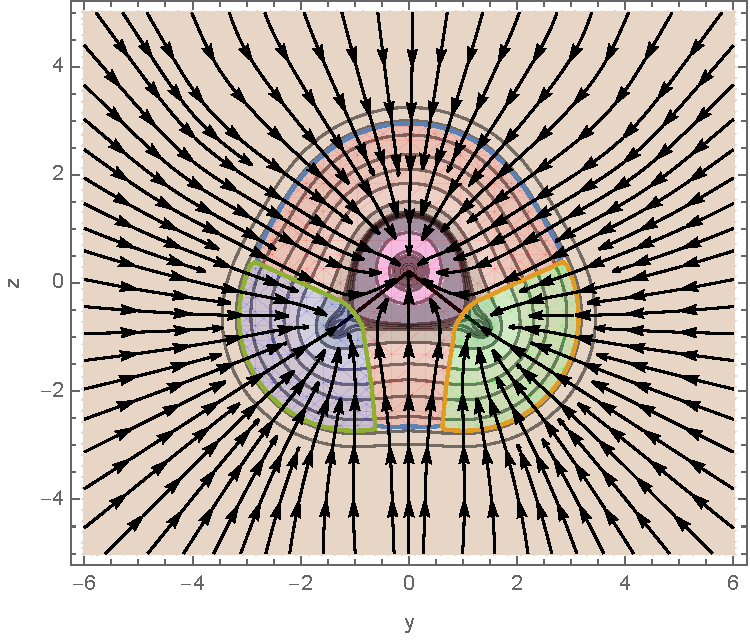
\includegraphics[width=0.65\textwidth]{./img/awa_basin}
  \caption{Atomic basins and gradient paths (black arrows) for the water
    molecule. The oxygen atom is shown in red, and the hydrogen atoms in green
    and blue. Blue, green, and orange contour lines represent zero-flux surfaces
    corresponding to the boundaries of the oxygen and hydrogen atomic basins.
    The orange background indicates regions excluded due to low electron density
    based on a threshold criterion.}
  \label{awaflux}
\end{wrapfigure}
%
\noindent where $\Omega$ denotes the atomic basin, $S(\Omega)$ the surface
bounding the basin, and $\mathbf{n}(\mathbf{r})$ the unit normal vector to the
interatomic surface at point $\mathbf{r}$. An atom in QTAIM is thus defined as
the union of a nucleus and its associated basin.

\vspace{1.4\baselineskip}%1.2
In summary, the spatial partitioning into disjoint Bader regions~\cite{bader} is
governed by the gradient vector field of the electron density, $\nnabla\rho(\mathbf{r})$.
This field defines a mapping $\mathbf{F} : \rreal[3] \to \rreal[3]$, which can
be analysed via its integral curves, or flux lines, given by the trajectories
$\sigma(t) : \rreal \to \rreal[3]$ defined in Equation~\ref{fluxlines}.

\vspace{1\baselineskip}%
As shown in Figure~\ref{awaflux}, the \gls{QTAIM} partition provides well-defined
spatial regions for each atom, enabling a detailed analysis of the system. The
classification of the associated \gls{CP} can then be carried out using
the scheme summarised in Table~\ref{PuntosCriticos}.

\newpage
\subsection{Topological Constraints and the Poincaré-Hopf Theorem}\label{phsection}

The Poincaré-Hopf theorem provides a deep connection between analysis and
topology. It relates the local behaviour of a vector field ---through its
\glspl{CP} and their indices--- to an invariant,
the Euler characteristic $\chi(M)$~\cite{Milnor1965}.

\thm{Poincaré-Hopf Theorem}{
  Let $M$ be a compact, connected, and smooth manifold, \& let $V$ be a tangent
  vector field on $M$ with isolated \glspl{CP}.
  Then the sum of the indices of the isolated \glspl{CP} is
  well defined and is equal to the Euler characteristic of $M$:

  \begin{align}
    \sum_{c \in CP} \text{index}(V, c) = \chi(M).
  \end{align}

  While the LHS of depends on a particular vector field, the RHS does not, \ie,
  although the individual indices vary with the choice of vector field, their sum
  is determined solely by the topology of the manifold. The Euler characteristic
  does not depend on the smooth structure of $M$, only on its triangualation, the
  topological structure of $M$.
}

In the context of \gls{QTAIM}, we are working with a partition of $\rreal[3]$
induced by the gradient vector field of the electron density,
$\nnabla\rho(\mathbf{r})$. The Poincaré-Hopf theorem can then be
used to establish a constraint involving the number and types of \glspl{CP} in
the system, providing a consistency check on any topological analysis of
\(\rho\).

The alternating sum over the number of \glspl{CP} of each index 
defines the Euler characteristic: $\chi(M) = \sum_{i=0}^{\max} (-1)^i M_i$ ,
where $M_i$ denotes the number of \glspl{CP} of index $i$.
For the case of a molecular system, the bounded region of 
$\rreal[3]$ under consideration is homeomorphic to the closed 
3-disk $D^3$, and thus $\chi(M) = 1$.
However, for a periodic system, by their boundary conditions,
the topological structure is that of
a 3-torus $T^3$, where the Euler 
characteristic is zero, $\chi(T^3) = 0$.

\begin{align}
  \chi(M) =
  \begin{cases}
    n_{\text{NCP}} - n_{\text{BCP}} + n_{\text{RCP}} - n_{\text{CCP}} = 1 \quad molecular \\
    n_{\text{NCP}} - n_{\text{BCP}} + n_{\text{RCP}} - n_{\text{CCP}} = 0 \quad periodic
  \end{cases}
\end{align}

\newpage
\subsection{Atomic properties in molecules}

In \gls{QTAIM}, the regions $\Omega$ correspond to atoms in the chemical sense,
and it can be rigorously shown that the postulates of quantum mechanics apply
within each of these atomic basins~\cite{bader}. Enforcing the zero-flux
condition on the gradient of the electron density yields a variationally
well-defined framework for assigning properties to each subsystem
independently~\cite{Bieglerknig1982}. Using the interatomic surfaces that
define the boundaries of these regions, molecular properties can be expressed
as the sum of the properties of the individual atomic basins:
%
\begin{equation}
  A = \sum_\Omega a_\Omega,
  \label{promoleculares}
\end{equation}
%
\noindent where $A$ denotes the total molecular property, and $a_{\Omega}$ is
the corresponding contribution from the atomic basin $\Omega$. This
decomposition is based on the atomic variational principle, which states that
if the operator $\hat{A}$ can be expressed as a sum of monoelectronic
operators, $\hat{A} = \sum\hat{a}$, then its expectation value can be written
as:
%
\begin{align}
  A(\Omega) &\equiv \langle\widehat{A}\rangle_\Omega \nonumber \\
    &= \int_\Omega\int\cdots\int\int\cdots\int
  \left [ \sfrac{N}{2}\Psi_{el}^{\star}\hat{a}\Psi_{el} + (\hat{a}\Psi_{el})^{\star}\Psi_{el}\right ]
  \dd\omega_1\ldots \dd\omega_N\dd\tau_2\ldots \dd\tau_N\dd\tau_1 .
\end{align}

This expression shows that an atomic property can be obtained by
integrating the expectation value of the corresponding operator over the atomic
basin $\Omega$.
To facilitate this, the concept of a local operator density is introduced. The
operator density $\rho_{A}(\mathbf{r})$ associated with $\hat{A}$ is defined as:
%
\begin{align}
  \rho_{A}(\mathbf{r}) = \sfrac{N}{2}\int\cdots\int\int\cdots\int[
  \Psi_{el}^{\star}\hat{a}\Psi_{el} + (\hat{a}\Psi_{el})^{\star}\Psi_{el}]
  \dd\omega_1\dd\omega_2\ldots \dd\omega_N\dd\tau_2\ldots \dd\tau_N ,
\end{align}
%
\noindent where the integration is carried out over all coordinates except
$\mathbf{r}$, which serves as the evaluation point of the density. The property
associated with a given atomic basin is then obtained by integrating this
density over the region:
%
\begin{align}
  A(\Omega)=\int_{\Omega}\rho_{A}(\mathbf{r})\dd\tau .
\end{align}

